\section{Universal Author Representations: Architecture}
\label{chp:stylometry_extensions:architecture}

\begin{figure*}
    \centering
    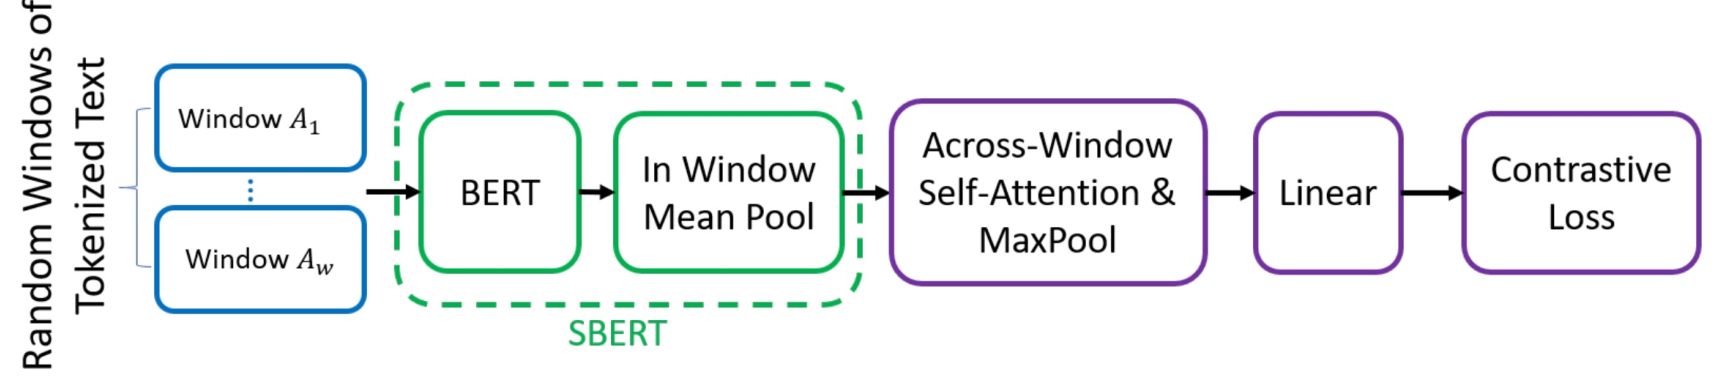
\includegraphics[width=\linewidth]{stylometryExtensions/figures/LUAR.pdf}
    \caption{Architecture for LUAR~\citep{riverastao2021learning}}
    \label{fig:stylometry_extensions:followingTrail:LUAR}
\end{figure*}

Figure~\ref{fig:stylometry_extensions:followingTrail:LUAR} shows the architecture for LUAR~\citep{riverastao2021learning}, the base author representation model used for exploring the research questions in this chapter. 
For an author $A$, given all the texts $T_A = \{t_1, \dots, t_{N_A}\}$ written by the author, each text is tokenized using the tokenizer corresponding to the transformer model used.
More details about tokenization strategies for different transformer models were provided in Section~\ref{sec:urltran:architecture:tokenization}.
An \textit{episode} is created by sampling contiguous windows of $l$ tokens from $w$ texts.
These windows are labeled $A_1, \dots, A_w$.
Each individual window is then encoded using a sentence transformer model~\citep{reimers2019sentencebert}.
A mean pooling operation is applied to the embeddings output by the final layer of the transformer model to generate a single vector representation for each window.
An additional mean-pooling operation is used to combine the representations of all windows to generate a single representation for the episode.
This representation is then transformed using a linear transformation and the final representation generated from this operation is used as the representation for one \textit{episode} for each author.
A supervised contrastive training loss~\cite{khosla2020supervised} is used a metric learning loss to ensure alignment between the embeddings of multiple episodes of the same author.
Further details about the training process and the loss function can be found in the LUAR paper~\citep{riverastao2021learning}.